\documentclass[
11pt,%
tightenlines,%
twoside,%
onecolumn,%
nofloats,%
nobibnotes,%
nofootinbib,%
superscriptaddress,%
noshowpacs,%
centertags]%
{revtex4}
\usepackage{ljm}
\usepackage{listings}
\usepackage{amsmath}

\lstset{
language=C++,
basewidth=0.5em,
xleftmargin=45pt,
xrightmargin=45pt,
basicstyle=\small\ttfamily,
keywordstyle=\bfseries\underbar,
numbers=left,
numberstyle=\tiny,
stepnumber=1,
numbersep=10pt,
showspaces=false,
showstringspaces=false,
showtabs=false,
frame=trBL,
tabsize=2,
captionpos=t,
breaklines=true,
breakatwhitespace=false,
escapeinside={\%*}{*)}
}

\begin{document}

\titlerunning{solving nonlinear equations}
\authorrunning{Bagrov, Rybakov}

\title{Selection of a Method for Solving Nonlinear Equations in Shallow-Water Icing Model Implementation}

\author{\firstname{A.~D.}~\surname{Bagrov}}
\email[E-mail: ]{andrey.bagrov@yandex.ru}
\affiliation{Joint Supercomputer Center of the Russian Academy of Sciences -- branch of Scientific Research Institute of System Analysis of the Russian Academy of Sciences, Leninsky prospect 32a, Moscow, 119334, Russia}

\author{\firstname{A.~A.}~\surname{Rybakov}}
\email[E-mail: ]{rybakov.aax@gmail.com}
\affiliation{Joint Supercomputer Center of the Russian Academy of Sciences -- branch of Scientific Research Institute of System Analysis of the Russian Academy of Sciences, Leninsky prospect 32a, Moscow, 119334, Russia}

\firstcollaboration{(Submitted by TODO)} % Add if you know submitter.
%\lastcollaboration{ }

\received{TODO}

\begin{abstract}
Моделирование ледяных наростов на профилях летательных аппаратов в процессе их полета в среде, содержащей переохлажденные капли воды, является крайней важной задачей для безопасности полетов, так как образуемые ледяные наросты существенным образом влияют на летные характеристики.
В одной из моделей решения поставленной задачи -- shallow-water icing model (SWIM) -- центральную роль в численном моделировании занимает задача решения нелинейных уравнений с одной переменной.
Так как данная задача занимает подавляюще большую часть всех расчетов, то вопрос выбора оптимального метода решения нелинейных уравнений и оптимизации данных методов встает особенно остро.
В данной статье описан анализ использования различных методов решения нелинейных уравнений в реализации решателя SWIM с учетом особенностей решаемых уравнений и продемонстрировано существенное ускорение расчетных кодов при выполнении вычислений на суперкомпьютерах МСЦ РАН.
\end{abstract}

\subclass{65H05, 65Y20} % Enter 2010 Mathematics Subject Classification.

\keywords{nonlinear equations, shallow-water icing model, метод бисекций, TODO}

\maketitle

\section{Introduction}

В настоящее время известно множество расчетных кодов, использующихся для численного моделирования обледенения поверхности обтекаемого тела.
Одними из наиболее популярных пакетов для решения данной задачи являются Lewice \cite{Wright} и ONERA.
В данной статье мы не будем касаться особенностей данных расчетных пакетов и различий между ними, а рассмотрим только реализацию решателя SWIM, подробно описанного в \cite{Bourgault}.
При выполнении компьютерного моделировании процесса обледенения поверхности, обтекаемой свободным потоком, в shallow-water icing model выполняется одновременный расчет нарастания льда и течения пленки жидкости по поверхности обтекаемого тела. При этом учитывается выпадение влаги на поверхность тела, испарение влаги или сублимация льда с поверхности тела, течение жидкой пленки по поверхности с частичным ее замерзанием, а также перетекание потоков тепла между телом и поверхностью и между поверхностью и окружающим воздухом.

Численные расчеты выполняются на поверхностной расчетной сетке, состоящей из отдельных ячеек, при этом в каждой ячейке поверхности должен выполняться закон сохранения массы, записываемый в следующем виде:

\begin{equation}
\rho_w \left[ \frac{\partial h_f}{\partial t} + \operatorname{div}(\overline{u} h_f) \right] = U_{\infty} LWC \beta - \dot m_{evap} - \dot m_{ice}
\end{equation}

В данной формуле $\rho_w$ -- плотность воды, $h_f$ -- высота водяной пленки на поверхности, $\overline{u}$ -- скорость течения водяной пленки, $U_{\infty}$ -- скорость набегания свободного потока, $LWC$ -- содержание влаги в набегающем потоке, $\dot m_{evap}$ -- удельная скорость испарения или сублимации с поверхности обтекаемого тела, $\dot m_{ice}$ -- удельная скорость нарастания массы льда.

Кроме того, в каждой ячейке выполняется закон сохранения энергии:

\begin{equation}
\begin{aligned}
& \rho_w \left[ \frac{\partial h_f C_w \tilde{T}}{\partial t} + \operatorname{div}(\overline{u} h_f C_w \tilde{T}) \right] = \left[ C_w \tilde{T}_{d,\infty} + \frac{||\overline{u}_d||^2}{2} \right] \times U_{\infty} LWC \beta
\\
& - \frac{1}{2}(L_{evap} + L_{subl}) \dot m_{evap} + (L_{fusion} - C_{ice} \tilde{T}) \dot m_{ice} + \sigma (T_{\infty}^4 - T^4) + \dot Q_h + \dot Q_{cond}
\end{aligned}
\end{equation}

В данной формуле $C_w$ -- удельная теплоемкость воды, $\tilde{T}$ -- температура ячейки в градусах Цельсия, $\tilde{T}_{d,\infty}$ -- температура выпадающей влаги в градусах Цельсия, $\overline{u}_d$ -- скорость выпадающих на поверхность капель, $L_{evap}$ - скрытая теплота испарения воды, $L_{subl}$ -- скрытая теплота сублимации льда, $L_{fusion}$ -- скрытая теплота плавления льда, $C_{ice}$ -- теплоемкость льда, $\sigma$ -- постоянная Больцмана, $T_{\infty}$ -- температура свободного потока в кельвинах, $T$ - температура ячейки в кельвинах, $\dot Q_h$ -- удельная величина потока тепла, получаемого из воздуха, $\dot Q_{cond}$ -- удельная величина потока тепла, поступающего в ячейку из обтекаемого тела.

Для численного решения приведенной системы уравнений необходимо выполнить ее дискретизацию по времени и пространстрву, как это показано в \cite{Beaugendre}.
После этого получим систему из двух разностных уравнений, в которые входят три неизвестные величины: температура поверхности $\tilde{T}$, высота водяной пленки $h_f$ и высота ледяного нароста $h_{ice}$.  

Также при решении системы уравнений должны выполняться условия совместимости, записываемые в виде

\begin{equation}
\begin{cases}
h_f \ge 0\\
\dot m_{ice} \ge 0\\
h_f \tilde{T} \ge 0\\
\dot m_{ice} \tilde{T} \le 0
\end{cases}
\end{equation}

\begin{figure}[h]
\setcaptionmargin{5mm}
\onelinecaptionstrue
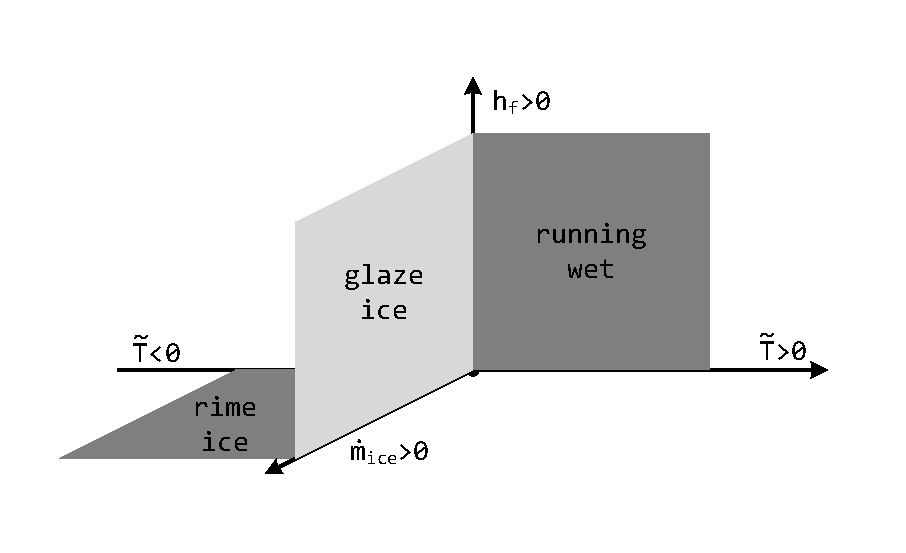
\includegraphics[width=0.7\textwidth]{pics/surface.pdf}
\captionstyle{normal}\caption{Пространство решение системы уравнений массового и теплового баланса ячейки.}\label{fig:surface}
\end{figure}

Несмотря на то, что неизвестных в уравнении больше, чем самих уравнений, система все равно решается, так как данные переменные не являются полностью независимыми.
Решение ищется из условия того, что ячейка может находиться в одном из трех состояний.
Первое состояние -- running wet -- достигается когда в ячейке полностью отсутствует лед и течет жидкая пленка.
В этом случае температура не может быть отрицательной.
Второе состояние -- glaze icing -- если в ячейке одновременно присутствует и лед, и вода.
В этом случае температура равна нулю градусам по Цельсию.
И наконец, в третьем случае при отрицательной температуре в ячейке не может находиться вода и присутствует только лед.
Общее пространство решений показано на Fig.~\ref{fig:surface}.

\section{Features of the equations being solved}

\begin{figure}[h]
\setcaptionmargin{5mm}
\onelinecaptionstrue
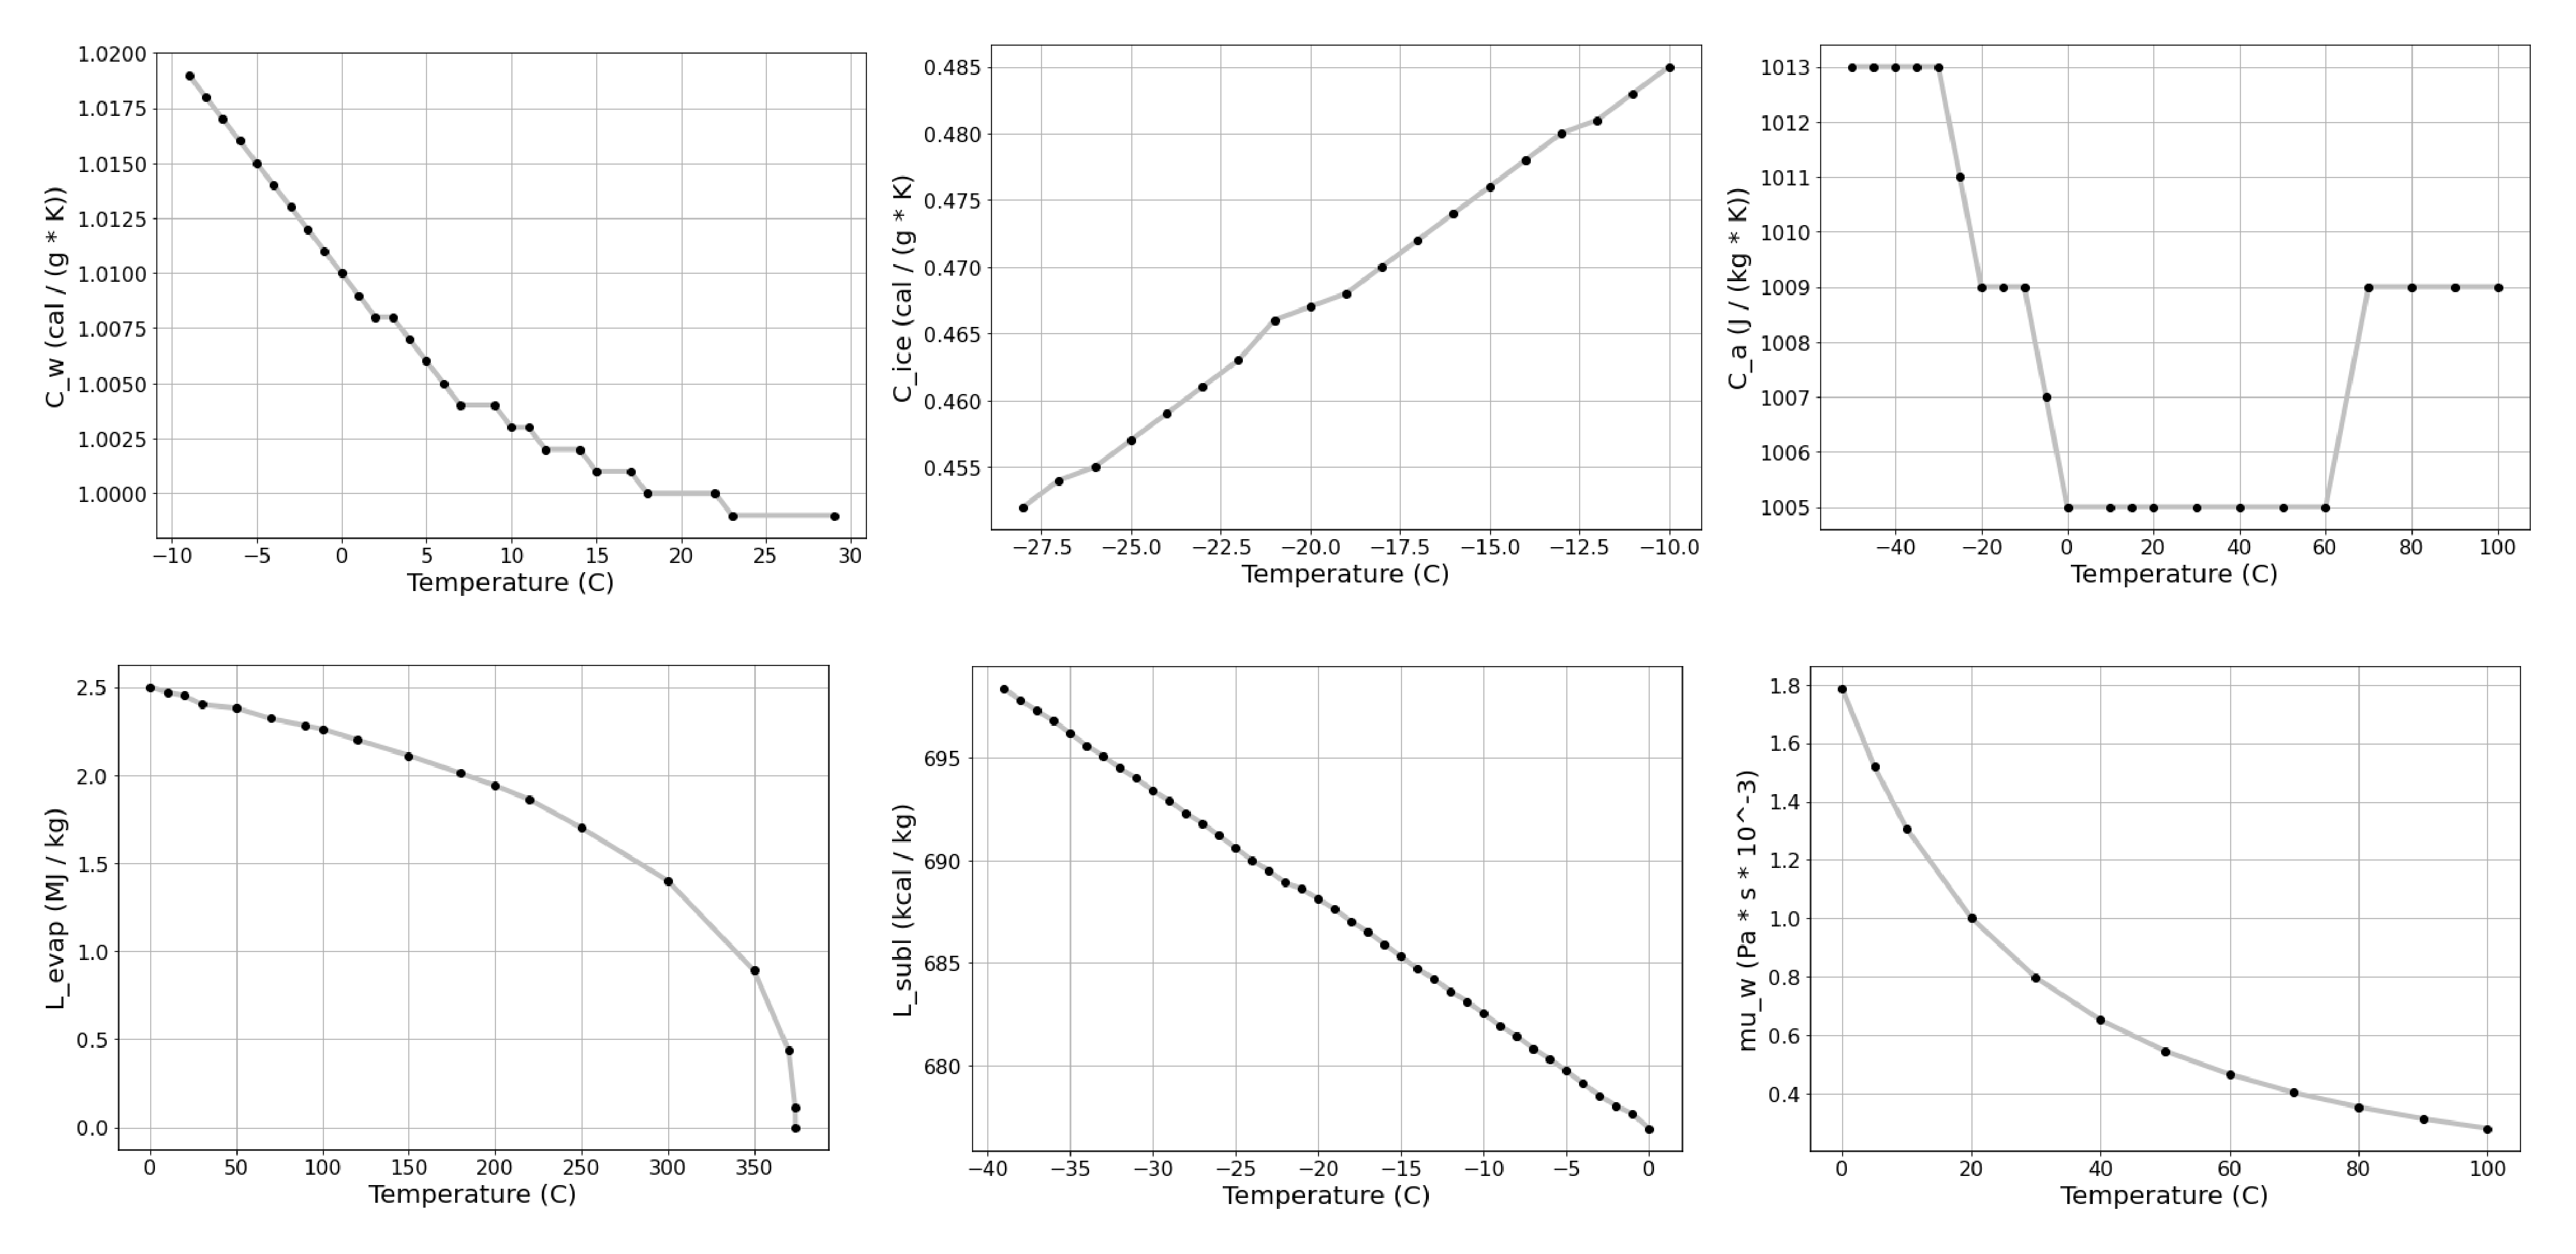
\includegraphics[width=1.0\textwidth]{pics/ph_graphics_h.pdf}
\captionstyle{normal}\caption{Зависимости физических величин от температуры.}\label{fig:surface}
\end{figure}

\begin{figure}[h]
\setcaptionmargin{5mm}
\onelinecaptionstrue
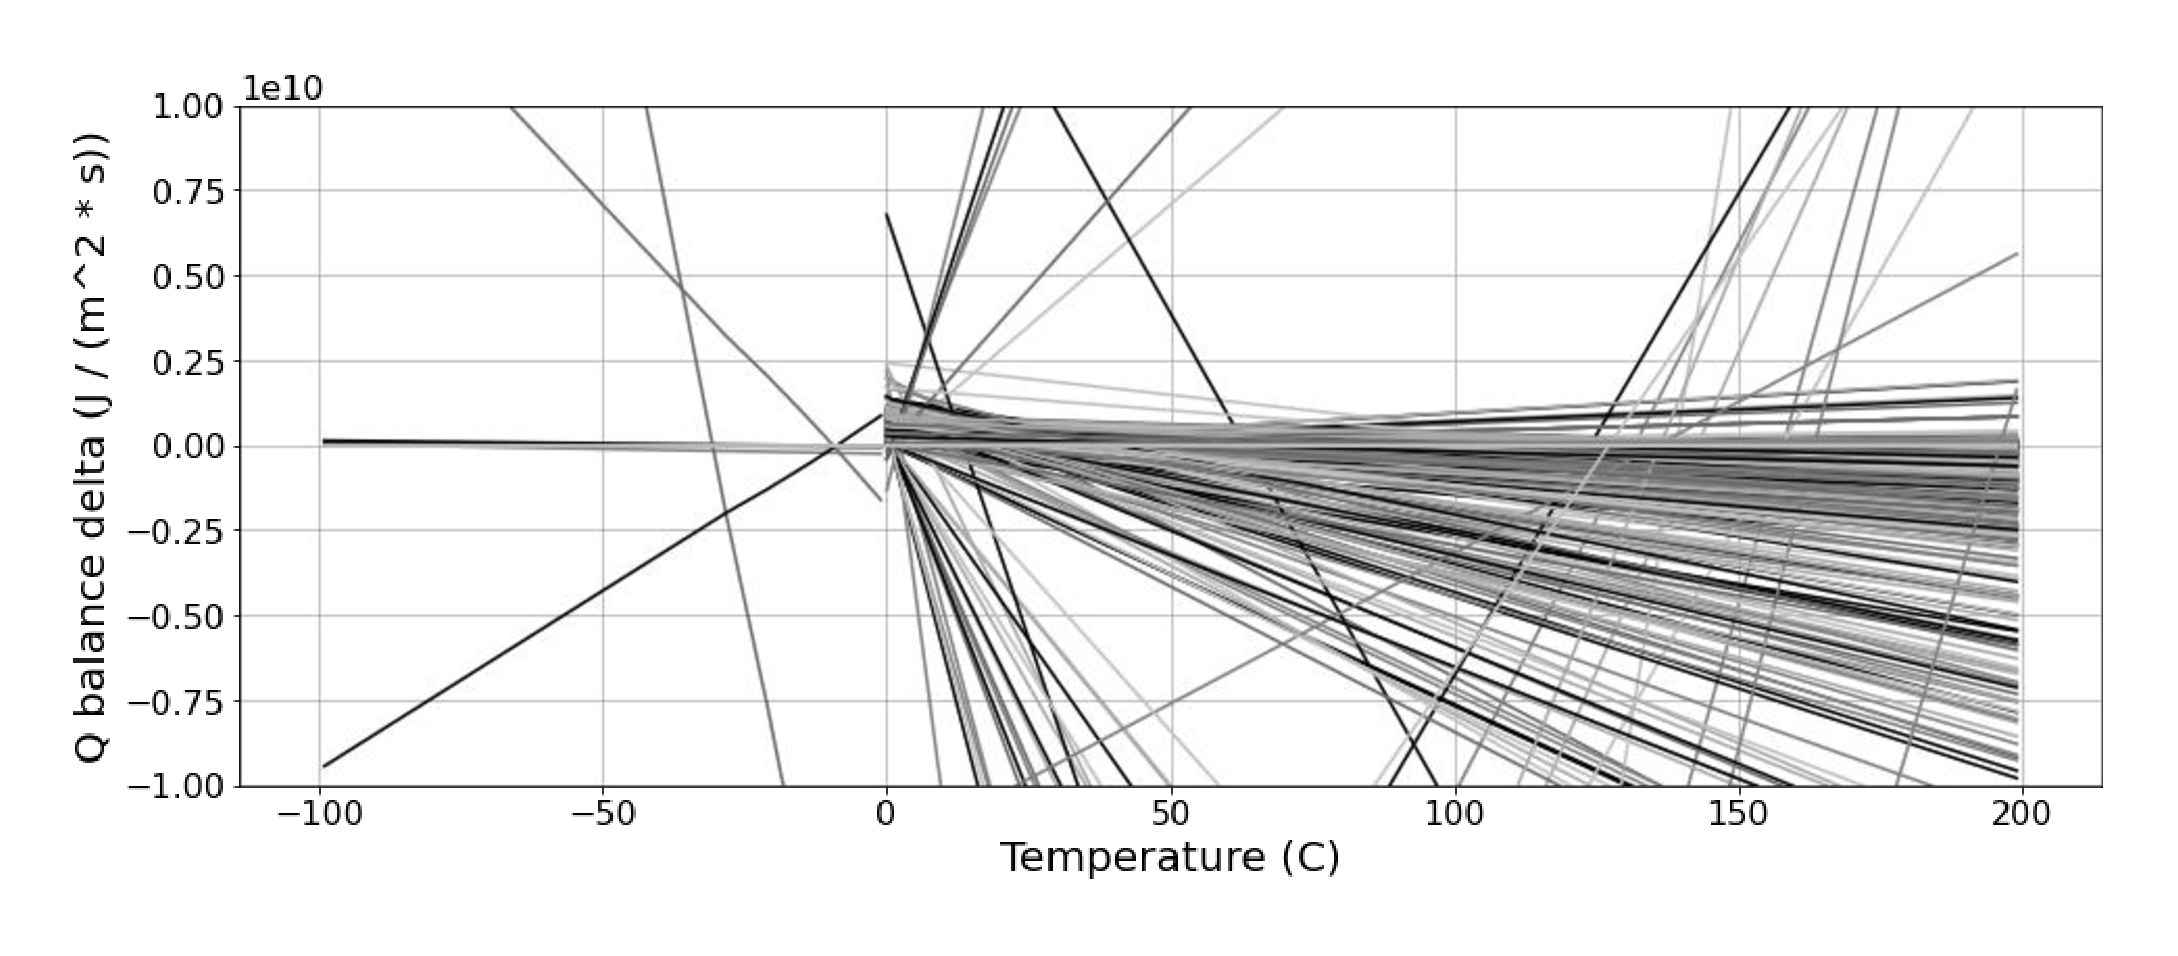
\includegraphics[width=1.0\textwidth]{pics/dq.pdf}
\captionstyle{normal}\caption{TODO}\label{fig:dq}
\end{figure}

\begin{figure}[h]
\setcaptionmargin{5mm}
\onelinecaptionstrue
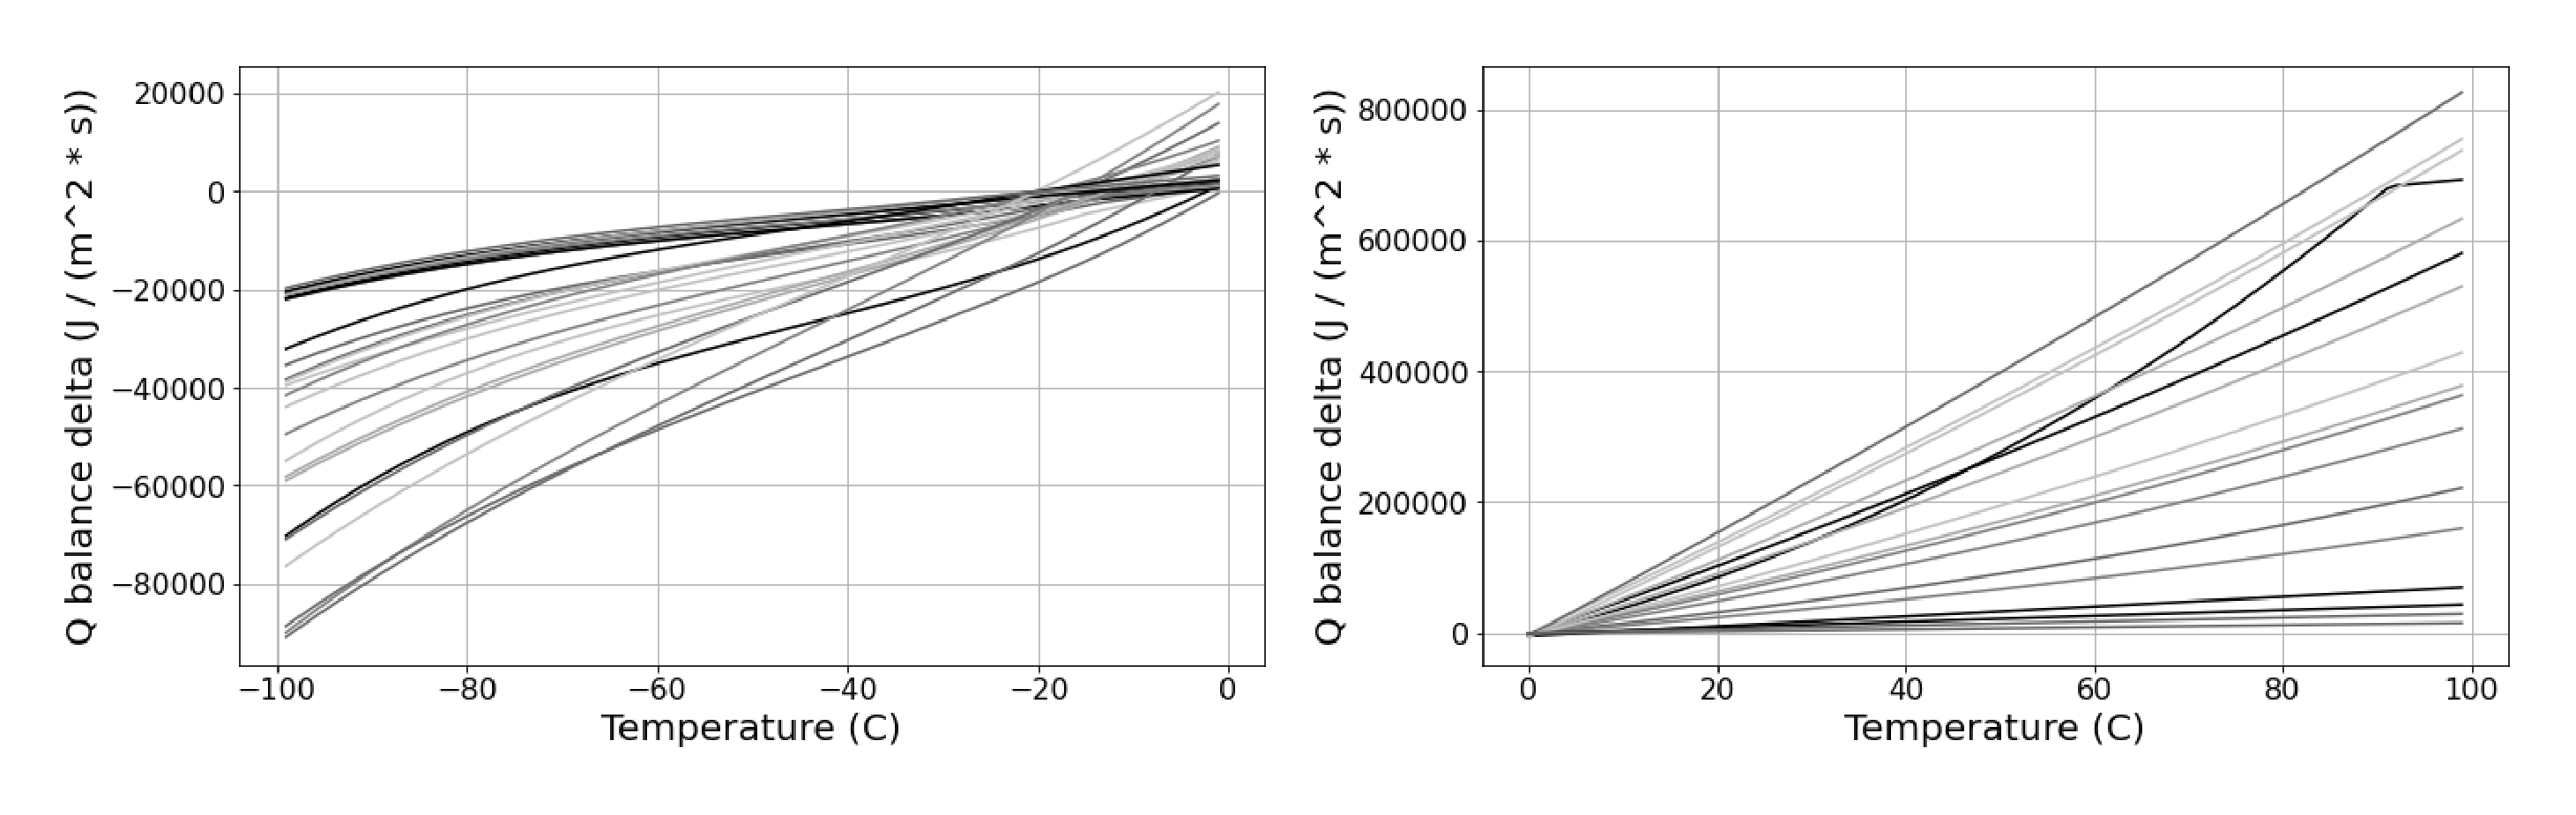
\includegraphics[width=1.0\textwidth]{pics/dq_rime_wet.pdf}
\captionstyle{normal}\caption{TODO}\label{fig:dq_rime_wet}
\end{figure}

\section{Methods of solving nonlinear equations}

TODO - на все методы нужна одна картинка, иллюстрирующая его и описание - один абзац, одна формула.

\section{Numerical experiments}

TODO

\section{Conclusion}

TODO

\begin{acknowledgments}
The work has been done at the JSCC RAS as part of the state assignment for the topic 0580-2021-0016.
The supercomputer MVS-10P OP, located at the JSCC RAS, was used during the research.
\end{acknowledgments}

\begin{thebibliography}{99}

\bibitem{Wright}
\refitem{articel}
W.~W.~Wright, P.~Struck, T.~Bartkus, G.~Addy, {\it ``Recent Advances in the LIWICE Icing Model''}, SAE Technical Paper (2015).

\bibitem{Bourgault}
\refitem{article}
Y.~Bourgault, H. Beaugendre, W. G. Habashi, {\it ``Development of a Shallow-Water Icing Model in FENSAP-ICE''}, Journal of Aircraft, Vol. 37, No. 4, 640--646 (2000).

\bibitem{Beaugendre}
\refitem{misc}
H.~Beaugendre, {\it ``A PDE-Based Approach to In-Flight Ice Accretion''}, A thesis of the degree of Doctor of Philosophy, Department of Mechanical Engineering, McGill University, Montreal, Qu\'ebec (2003).

\end{thebibliography}

\end{document}
